\section{Background}

\subsection{Explainable Artificial Intelligence (XAI)}

The field of XAI research is still very far behind it's counterpart AI research,
within XAI two fields are concidered the largest that is Model Interpretability
and Model Explainability.

\subsubsection{Model Interpretability}

\subsubsubsection{Saliency Maps}
Within XAI many methods have been developed to try to evaluate
ANN's, these methods are often referred as model interpretability methods.
In the field image recognition there has been a lot of work examining which
pixels of an image the model deems important. Arguably the most popular
method for this is Saliency Maps (CITE ME). There the pixel values the model
deems important are colored in s.t. a human can examine the image and get a
sense of what portions of the image are important to the model, an example of
a classification of a dog can be seen in Figure \ref{fig:dog_saliency}.

\begin{figure}[]
  \centering
  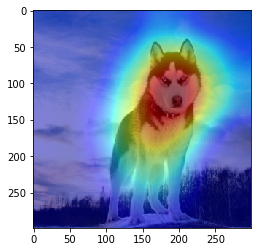
\includegraphics[width=.5\textwidth]{graphics/dog_saliency}
  \caption{Example of a models saliency map for an image of a dog}
  \label{fig:dog_saliency}
\end{figure}

While this method is understandable in the context of image recognition it
lacks severely when your input is not an image.

\subsubsubsection{Shapley Values}

Methods for explaining models that aren't image recognition models include
shapley values. There the input is examined against it's output, then iteratively
input values are selected to be fixed. Then the other input values are varied and
an average change in prediction is calculated. With this the shapley value can be
estimated for the fixed input value. This is done to examine which input values have
the strongest link to the output value. Shapley values on a dataset can give insights
on which input values the model deems important.

\subsubsubsection{Concept Activation Vectors}

A recent paper by Been Kim Et. al (CITATION NEEDED), shows a method for examining
a neural network giving a much more human insight into a prediction. Using Concept
Activation Vectors (CAV) a directional derivative for a given input can be examined
with respect to some HLC's. For example, when a human looks at an image of an animal
and is supposed to decide whether the image is of a horse or a zebra, an intuitive
approach would be to check whether the animal has stipes, or is both white and black.

CAV's in neural networks are just binary classifiers of the same dataset used to train
a neural network. The 

\subsubsection{Model Explainability}

Model explainability within the context of neural networks isn't possible today. Model
explainability referrs to firstly considering some input and output from a model. Then
afterwards the model is examined to determine exactly what led to the predicted output.
This concept is simple when we're working with Decision Trees. A decision tree is a tree
whose nodes are representative of an input value and at every node a branch is selected
based on the value of the input value. It is therefore easy to see how to examine the tree
to explain the output. We just follow the branches in the tree. That being said the branches
are created by algorithms like ID3 which construct branches based on the initial dataset used
to construct the tree, but again ID3 follows simple statistics and can be explained properly.

When we talk about neural networks this process is much more difficult, the underlying nodes
are generally in the thousands, the different layers of the neural network varies in the operations
it applies to the input value and such while travelling through the neural network the modified
value becomes far removed from the initial input value to the eyes of the reader. That being said,
while the possibility of completely monitoring the training process and completely monitoring the
evaluation process is truly possible it is not feasible. And secondly the process of seeing an
input and it's corresponding output will not be of any value if one were to consider the process
of prediction.

\subsection{Machine Learning}

\subsubsection{Reinforcement Learning}

Reinforcement Learning is a subfield of Machine Learning where a model learns from experience.
That is, the notion of input/output values changes, the model uses itself to generate input
values by acting in an environment. The environment then returns some result, that could be
losing in a game, making a correct prediction, or any number of outcomes. The result is then
propagated through the model moving it's parameters in the direction of the recieved output
from the environment.

Many algorithms are popular in reinforcement learning, for instance Q-learning(CITE ME), CARLA (CITE ME),
Monte Carlo Tree Search, and many others. The work in this paper relies heavily on Monte Carlo Tree Search,
and will be the only one thoroughly discussed.

\subsubsection{Monte Carlo Tree Search}

In the algorithm Monte Carlo Tree Search there is an agent exists
within some environment. Where each node in the environment represents a state-action pair of the environment, by
state-action pair what is meant it is some state and the action that brought the agent to
that state. This pair should be unique within the environment. We will discuss these concepts within game-environments
and therefore we might say player instead of agent and game instead of environment.

Monte Carlo Tree Search is a method of exploring an enviroment in a randomized manner (Monte Carlo is the term implying
randomness). In MCTS there are four stages. Selection, Expansion, Simulation, and Backpropagation. They happen sequentially
and repeatedly. MCTS is initialized with a tree consisting of the unexpanded initial state of the environment.

In MCTS there is a tree representing the game-environment. This tree consists of nodes $n_i$ where $i$ represents the point in time
of the node, for example $N_0$ in chess is the initial position and $N_x$ is some position in the middle of the game and $N_e$ is one of
the states representing a position where there is either a draw or one player has won the match. Each of the nodes has $4$ values,
$s$, $a$, $Q$, and $N$. These values represent these items, $s$ is state of the environment, $a$ is the action that brought
the previous node $n_(i-1)$ to node $n_i$, $Q$ is the average value of the node (value meaning the outcome of the game),
and $N$ the amount of times the MCTS algorithm has visited this node. The values $s$ and $a$ uniquely identify a position
in the environment and are often called state-action pairs.

The MCTS algorithms four phases
\begin{enumerate}
  \item Selection
  \item Expansion
  \item Simulation/Rollout
  \item Backpropagation
\end{enumerate}


\begin{equation} \label{UCT_formula}
  \text{Child UCT value} = \frac{Q_{(s',a')}}{N_{(s',a')}} + c_{uct} * \frac{\sqrt{log(N_{(s,a)})}}{N_{(s',a')}}
\end{equation}

\subsubsection*{Selection}
During the selection phase a node $(s,a)$ within the tree which has not yet been expanded is found.
This process uses Upper Confidence Bound on Trees (UCT) to find that node $(s,a)$, the formula is described in Equation \ref{UCT_formula}. For a parent node $(s,a)$
(initially the root of the tree) we select the child with the highest UCT value. Repeatedly until an unexpanded
node is found. This process is done to balance the amount of exploration vs exploitation of nodes in the
tree.

\subsubsection*{Expansion}
Then the expansion phase expands the node generating all of $(s,a)$'s children $(s',a')$ are generated
and connected to $(s,a)$. This is done by applying all actions $a'$ to $(s,a)$. These children are the
product of applying each action $a'$ to $s$ in the parent node.

\subsubsection*{Rollout}
Next during rollout actions from $(s,a)$ are randomly selected to move to $(s',a')$, then repeated
to go to $(s'',a'')$, until a terminal node within the environment is reached. By terminal we mean a
state in which the game is finished. A terminal node in MCTS can generally return any value, but in the
context of this paper we only return (+1 white wins, -1 black wins, 0 draw).


\subsubsection*{Backpropagation}
The result from the terminal node is then propagated up through the path taken by selection $(s,a)$ up
to the root of the tree, updating the $Q_{(s,a)}$ values of each node $(s,a)$.

When training a neural network the UCT formula is modified slightly to prefer selecting nodes
that the neural network values highly by introducing a second scalar to the formula $f(s,a) = (p,v)$,
the resulting formula is described in Equation \ref{PUCT_formula}, and is called PUCT. Secondly, the backpropagation process
is modified to instead of doing rollout/simulation to recieve a reward the predicted value $v$ from
the neural network is used instead.

\begin{equation} \label{PUCT_formula}
  \text{Child PUCT value} = \frac{Q_{(s',a')}}{N_{(s',a')}} + c_{uct} * P((s,a)) * \frac{\sqrt{log(N_{(s,a)})}}{N_{(s',a')}}
\end{equation}

